\section{Formative Work: Understanding Creative Live Streams}
\label{sec:liveclips_formative}
Creative live streams are a unique and rapidly growing source of data that have yet to be deeply studied.  To understand the current landscape of creative live streams as well as their applicability to inspiration in software, we conducted content analysis, interviews, and surveys, exploring the following three questions:

\begin{enumerate}
    \item \textbf{What are creative live streams?} For a general sketch of creative live streams, we present a content analysis of a sample of live streams that illustrates the range of content people stream and the different types of creative live streams.
    \item \textbf{Why and how do people stream creative work?} Which parts of their process do they stream? To understand streamers' motivations, processes, and challenges, we present findings from interviews with 8 creative streamers and compare their experiences with streamers in other domains.
    \item \textbf{Why do people watch creative live streams?} To understand the audience these streamers reach, we present findings from three online surveys with 165 viewers that highlight learning and inspiration as key motivators, with entertainment and community close behind.
\end{enumerate}

We found that viewers often seek to learn and be inspired from creative live streams. Notably, inspiration is a much more prominent theme compared with prior work in other live streaming domains such as gaming. However, many streaming platforms are not designed to support these goals, and watching archived streams is tedious. These findings further motivate our goal to make live streams available to users in the context of their own workflows.

\subsection{What Are Creative Live Streams?}
Live stream videos (\autoref{fig:livestreaming_view}) typically show the artist's full screen (when working on a computer) or workspace (for physical work) and a camera view of their face. Live streams usually also feature a live chat, allowing viewers to communicate with each other and the artist. 

There are two main things that make live streamed videos different from other types of videos demonstrating creative work, such as tutorials. First, live streamed videos usually show a real-world process, imparting both creative and procedural knowledge, while tutorials often show contrived tasks, and impart mainly procedural knowledge \cite{Torrey2007}. Second, artists often start without an exact goal in mind, and it can be inspiring to watch someone go from a blank canvas to a beautiful piece of work, though this also means watching the less ``glamorous'' parts of the creative process such as silent thinking or tedious, repetitive tasks.

To learn more about creative live streams, we studied two popular platforms: Twitch and YouTube. As these large platforms cover many types of content, we narrowed our investigation to the \textit{Creative} category on Twitch and the \textit{Adobe Live} video series on YouTube. Through this, we see how streams and communities differ across platforms.  

\begin{figure}[b!]
\centering
  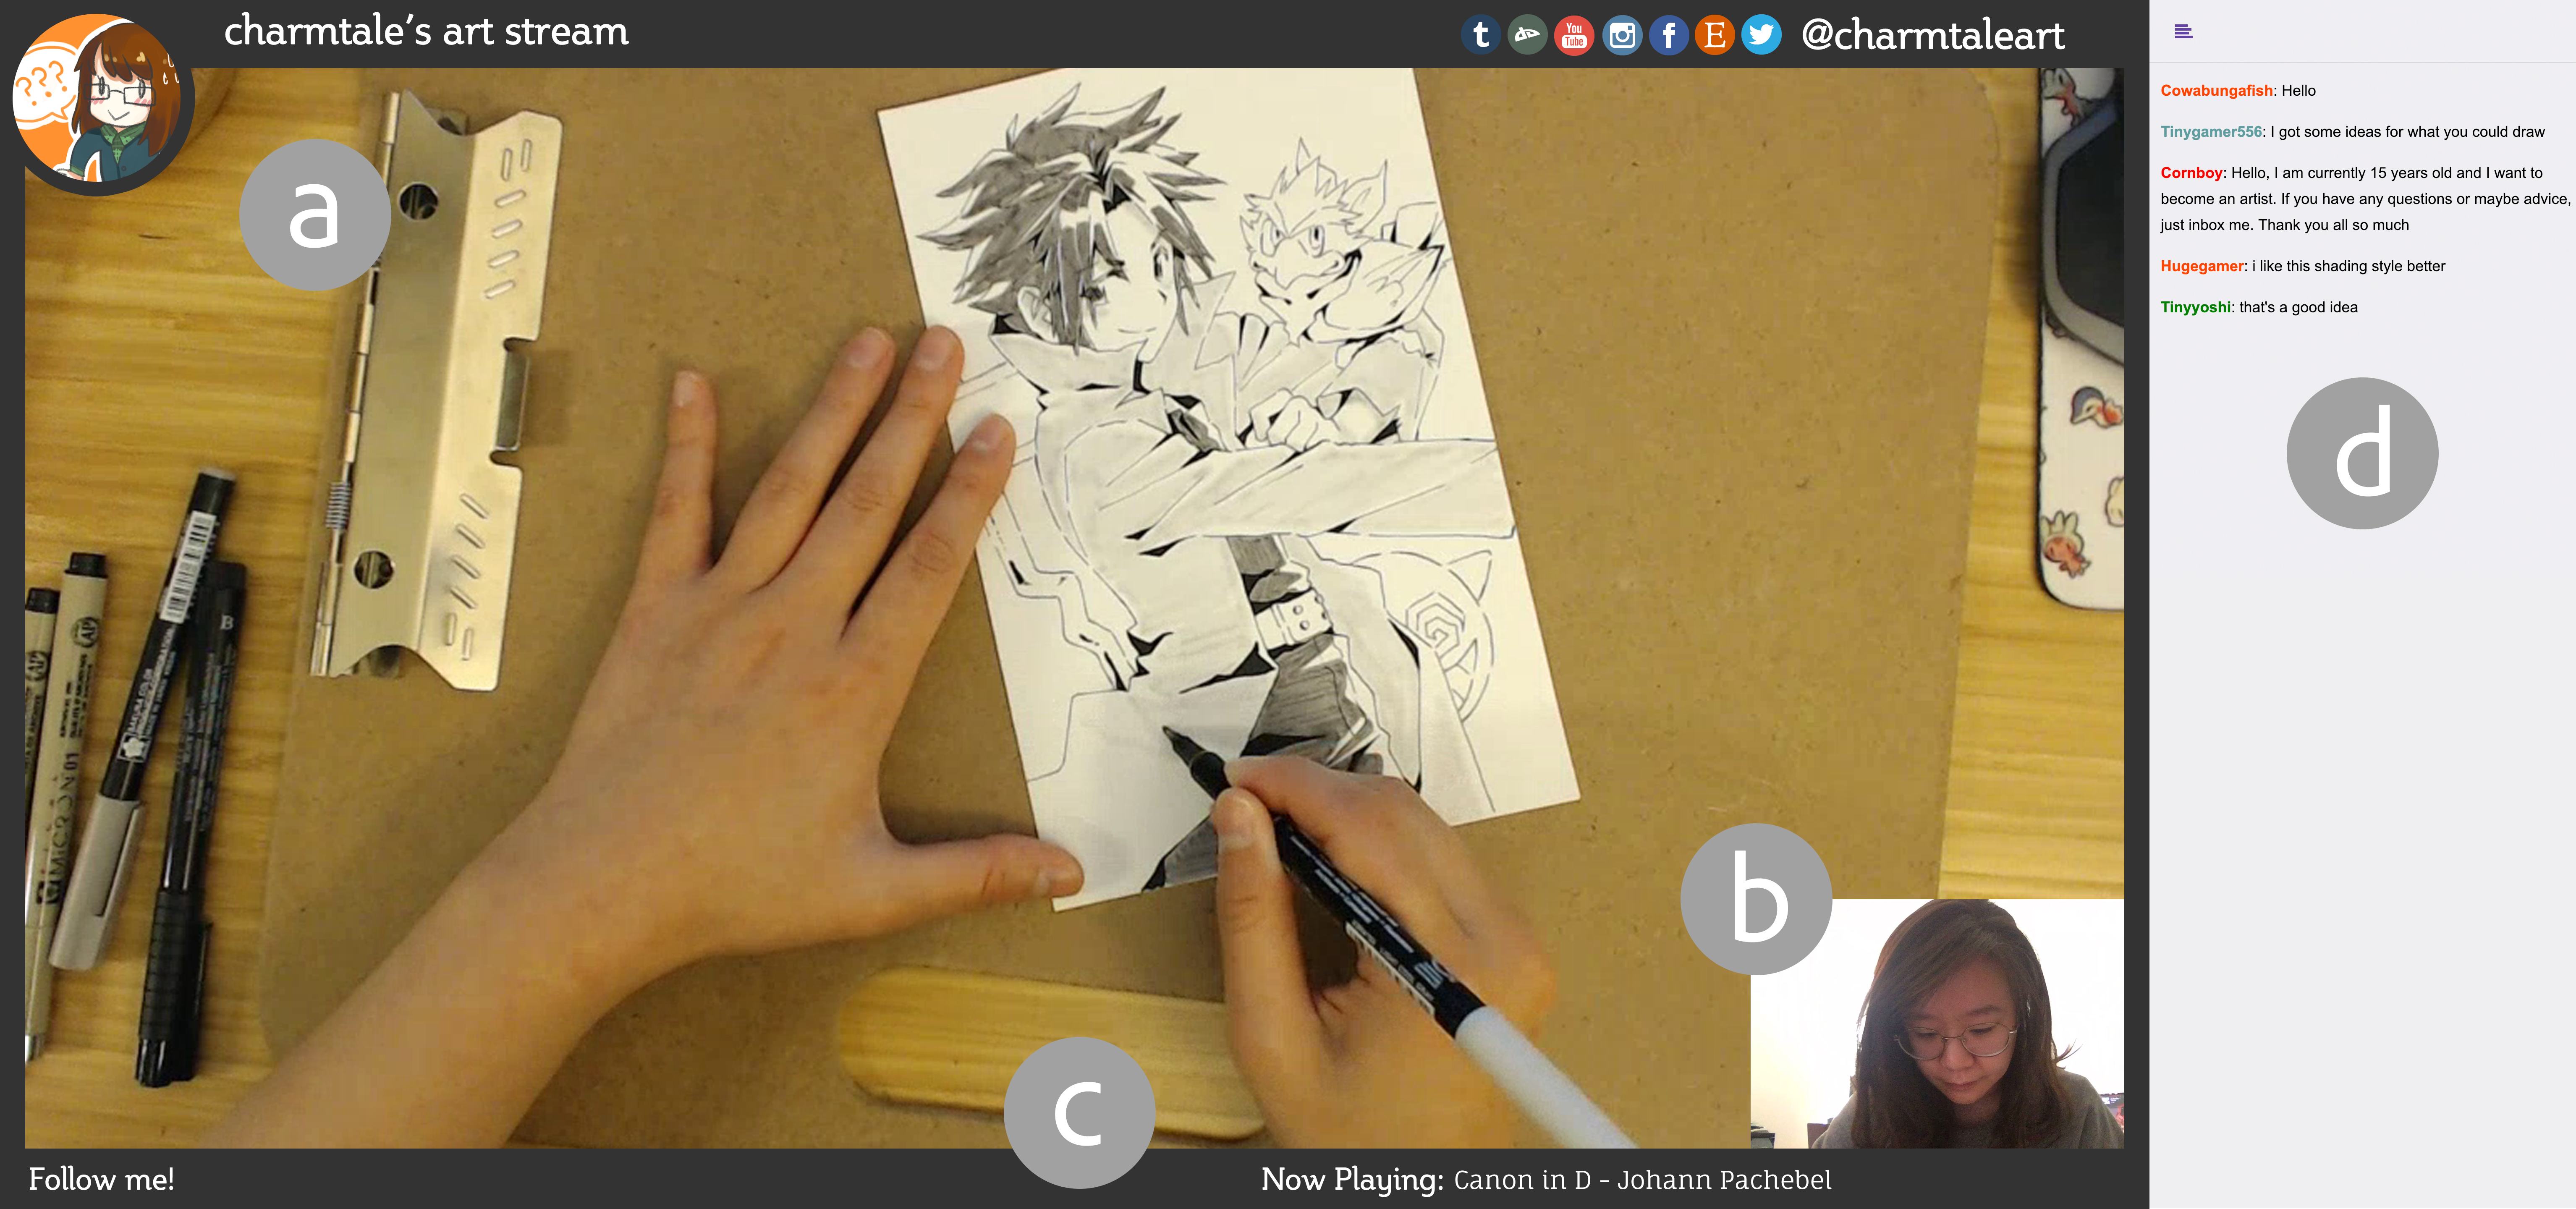
\includegraphics[width=0.7\columnwidth]{liveclips/figures/livestreaming_paper_figure_anonymized.jpg}
  \caption[A typical creative live stream setup.]{A typical creative live stream setup. (a) A camera or screencast displays the artist's workspace. (b) A second camera shows the artist's face. (c) Graphical overlays provide ambient information about the artist (\textit{e.g.}, social media pages) and display interactions with the audience (\textit{e.g.}, pop-ups that appear when viewers subscribe or donate to the stream). (d) Live chat allows viewers to communicate with the streamer. }~\label{fig:livestreaming_view}
\end{figure}

\subsubsection{Creative live streams on Twitch: Content analysis}
To better understand the format and content of creative live\-streams, we analyzed a sample of videos on Twitch, one of the most popular platforms for live streaming. For each creative category, we gathered aggregate metrics about streamers and viewers. We watched and took notes on a sample of 29 videos. We identified four common types of creative live streams that will appear throughout the chapter: \textit{Teaching}, \textit{Making}, \textit{Socializing}, and \textit{Performing}.

\textbf{Methodology:}
To measure the popularity and activity in each of the six creative categories, we queried the Twitch \textsc{api} 4 times a day for 7 days to obtain the number of currently-live streams and number of currently-watching viewers in each category.

We also used the Twitch \textsc{api} to download metadata about the videos in each category (limited to top 600)
%Because this \textsc{api} halts video requests after 600 videos, so our script downloaded metadata for the 600 most-viewed videos in each category. The script 
and randomly selected 50 archived English live stream videos. Four annotators (including the first author) watched each of these videos. Ten videos were not available for viewing and thus excluded (either because their archive expired between being downloaded and being annotated, or because they were only available to subscribers of a channel). Another 11 videos were excluded as they showed video games, TV show reruns, or live event coverage. While these videos were categorized as creative on Twitch, they did not reflect our definition of creative work, namely the creation of a novel artifact. This yielded 29 videos. For each, annotators took notes in a structured spreadsheet on the content presented, camera setup, overall structure of the stream, artist's presentation style, and chat activity.

\begin{table}[t]
\centering
\caption{Summary of popularity of Twitch's creative live stream categories. The number of currently-live streams and currently-watching viewers were collected 4 times a day for a week and then averaged.}~\label{table:livestream_summary}
\begin{tabular}{llll}
\textbf{Category}        & \textbf{\begin{tabular}[c]{@{}l@{}}Avg. \#\\ live streams\end{tabular}} & \textbf{\begin{tabular}[c]{@{}l@{}}Avg. \# live\\ viewers\end{tabular}} & \textbf{\begin{tabular}[c]{@{}l@{}}Avg. \# viewers\\ / stream\end{tabular}} \\
Art                      & 339                                                                    & 6417                                                                    & 21                                                                          \\
Beauty \& Body Art       & 5                                                                      & 177                                                                     & 17                                                                          \\
Food \& Drink            & 19                                                                     & 1088                                                                    & 64                                                                          \\
Makers \& Crafting       & 40                                                                     & 680                                                                     & 16                                                                          \\
Music \& Performing Arts & 286                                                                    & 6881                                                                    & 24                                                                          \\
Science \& Technology    & 91                                                                     & 1155                                                                    & 12                                                                         
\end{tabular}
\end{table}

While this sample does not capture all types of creative activities one might live stream, our hope is that by analyzing a set of canonically creative activities we can shed light on a broader set of activities that might also have a creative component (\textit{e.g.}, video games that involve creating artifacts).
%There is overlap among categories on Twitch, even sometimes within a single live stream when an artist switches back and forth between creative work and other activities like gaming. 

\textbf{Results: Most streamers focus on work \& engage with viewers:}
\autoref{table:livestream_summary} shows overall metrics for the creative categories on Twitch. The most popular categories by far are \textit{Art} and \textit{Music \& Performing Arts}. The category with the most viewers watching per stream is \textit{Food \& Drink}, likely because there are fewer streams to choose from relative to the number of interested viewers. These communities are small relative to the most popular games; for example, the game Fortnite has between 5,000 and 10,000 streams live on Twitch at any given time, with around 100,000 total viewers watching. %\xxx{xxx says move earlier but where?}

\begin{table}[t!]
\centering
\caption{Creative activities shown in a random sample of 29 live streams from Twitch's creative categories, and the primary type of structure each stream exhibits.}~\label{table:livestream_activities}
\begin{tabular}{lll}
\textbf{Category}        & \textbf{Activity (\# videos if \textgreater 1)} & \textbf{\begin{tabular}[t]{@{}l@{}}Primary type\\ of stream\end{tabular}} \\
Art                      & Multimedia production                           & Making                                                                    \\
                         & Digital drawing (4)                             & Making                                                                    \\
                         & Animation                                       & Teaching                                                                  \\
                         &                                                 &                                                                           \\
Beauty \& Body Art       & Makeup                                          & Socializing                                                               \\
                         & Makeup (3)                                      & Making                                                                    \\
                         &                                                 &                                                                           \\
Food \& Drink            & Cooking                                         & Teaching                                                                  \\
                         &                                                 &                                                                           \\
Makers \& Crafting       & Making foam props                               & Teaching                                                                  \\
                         & Sewing quilts                                   & Socializing                                                               \\
                         & Bead art (2)                                    & Making                                                                    \\
                         & Assembling models                               & Making                                                                    \\
                         & Assembling models                               & Socializing                                                               \\
                         & Woodworking                                     & Making                                                                    \\
                         & Pottery                                         & Making                                                                    \\
                         &                                                 &                                                                           \\
Music \& Performing Arts & Music production                                & Performing                                                                \\
                         & Music production                                & Making                                                                    \\
                         & Acting \& improv games                          & Performing                                                                \\
                         &                                                 &                                                                           \\
Science \& Technology    & Building a computer                             & Making                                                                    \\
                         & Programming (3)                                 & Making                                                                    \\
                         & Game development (2)                            & Teaching                                                                  \\
                         & Talking about technology                        & Socializing                                                              
\end{tabular}
\end{table}

The videos span a range of creative activities (\autoref{table:livestream_activities}). The average video length was 3h46m, not including time spent gaming -- a few artists combined both creative work and video gaming into one stream, spending the first part on creative work then switching to gaming when they were finished. The shortest video was 1h3m; the longest was 7h56m. These videos are notably longer than most non-live-stream videos.

Almost all videos contained either a screencast view for work being done on a computer (13/29) or a camera view for physical work (15/29). One showed a distant camera view of the artist producing music in a studio. Most (26/29) showed the artist's face: in 10 as part of the main camera feed, and 16 as a separate feed overlaid in a corner (as in \autoref{fig:livestreaming_view}). Almost all artists (27/29) talked out loud while streaming; of the two silent streamers, one occasionally posted in the chat. Most artists talked about a mix of their work and other topics (18/29). Some talked only about their work (9), or only about other topics (1). One was a variety show, so the talking \textit{was} the work. Many videos (19/29) included background music. 

Most artists engaged with the chat at least sometimes (24/29). 18 artists engaged frequently with the chat, and 6 occasionally. Three videos did not show a chat replay despite the artist referring to the chat; we assume it was not saved or had been hidden. In all 26 remaining videos, viewers asked questions at least occasionally, or in some videos (9/26) frequently. In half of these videos, all chat questions appeared to get answered; in the rest, some (7/13) or many (4/13) questions went unanswered. In 2 videos, most chat questions were answered by other viewers or moderators in the chat.

\textbf{Four common types of creative live streams:}
We identified four common types of creative live streams. We also observed these in interviews with streamers in the next section. Sj{\"{o}}blom \textit{et al.} \cite{Sjoblom2017a} offer a similar characterization of video game live streams; we found some key differences and fewer overall types of structures. \autoref{table:livestream_activities} shows the primary type of each stream in our sample set. These are general high-level trends; some streams bridge multiple types.

\textbf{Teaching} streams have an instructional focus, where the stream\-er is educating the viewers. These include step-by-step how-to demonstrations of tasks such as cooking a recipe, producing a photo-editing effect, or creating DIY costumes. Other examples include critiquing others' work, answering viewers' questions, or explaining a topic.

\textbf{Making} streams focus primarily on creative work and process, but not explicit teaching. These include an artist silently drawing, a streamer attempting a new task they have not tried before and talking their way through it, and an artist making pottery and describing \textit{what} they are doing but not \textit{how}. 

\textbf{Socializing} streams feature the streamer chatting casually with viewers, often while working on a project, such as makeup or sewing (but the project is not the main focus). These are often described as ``chill'' streams. Socializing streams often have tight-knit communities; the streamer will recognize the names of viewers in the chat and ask them how they are doing.

\textbf{Performing} streams feature the artist performing their work. Naturally, these mostly include performative arts like music and acting (\textit{e.g.}, as opposed to drawing). Like with Making, the focus is on the artist's work; in this case the artist does not talk about what they are doing, they just do it. Performing streams differ from non-live recordings in that they often take a more casual improvisational form, rather than scripted performance (\textit{e.g.}, musical ``jam sessions'' or improv acting).

Within each type, the amount of interaction between the stream\-er and the audience varies. Some streamers hold ``request streams'' or ``Q\&A streams'', where the content and flow are determined by audience requests or questions, respectively. Some hold contests or games. A request stream could have audience members requesting songs for a Performing stream, a topic for a Teaching stream, or a particular artifact for the artist to make in a Making or Socializing stream. 

\subsubsection{Creative live streams go professional}
While many live streams are run by individuals, professionally-run streams are also growing in popularity. Adobe, a company that produces creative software, hosts live streams on a regular schedule multiple times a week\footnote{\href{https://behance.net/live}{\nolinkurl{behance.net/live}}}. These can be viewed on Behance or on Adobe's Creative Cloud YouTube channel. They host two live stream series: \textit{Adobe Live} is a Making stream that happens for 6 hours (three 2-hour sessions) three days a week, and it features guest artists usually hosted by someone who works at Adobe. \textit{Daily Creative Challenges} is a Teaching stream that happens for 30 minutes five days a week. It complements contests organized by Adobe to teach new skills. YouTube reports these streams having between 2,000 and 8,000 views each; it does not distinguish between live and replayed views.

\stepcounter{footnote}
\begin{figure}[b!]
\centering
  \includegraphics[width=0.6\columnwidth]{liveclips/figures/adobelive.png}
  \caption{The \textit{Adobe Live} series features a guest artist (bottom left) and a host (bottom right). The artist is working on a digital drawing, and the host is looking up at the live chat feed, engaging with the audience (\href{https://youtu.be/yYDmQhg_1uE}{\nolinkurl{youtu.be/yYDmQhg_1uE}}). }~\label{fig:livestream_adobelive}
\end{figure}

\textit{Adobe Live} differs from most streams by featuring two people. Typically there is a host and an guest artist (\autoref{fig:livestream_adobelive}), but sometimes two artists work together. Adobe hosts different artists every week across a range of creative disciplines (\textit{e.g.}, graphic design, UX design, photography, video editing). Typically, the host moderates the stream, responding to chat messages and passing on questions from viewers to the artist so that the artist can focus on their work. When the stream includes two artists, they trade off hosting.
%xxx: removing for now because we haven't talked about challenges for streamers yet
%These live streams address some of the challenges self-streamers often face, such as facilitating the chat while working and dealing with technical setup, by having separate people take on those tasks. 
The featured artists are usually practitioners, not teachers; their work mainly serves as inspirational demonstrations, while also giving the the community a chance to engage with questions and comments. 

The \textit{Daily Creative Challenges} series features one person who both reads chat messages and provides a short tutorial on a software technique. These live streams are part of Adobe's Creative Challenges, which are contests that encourage people to use Adobe software and submit design work for prizes\footnotemark. These streams are 30 minutes long -- this is short for a live stream -- and focus on instruction: explaining the challenge of the day and teaching viewers the skill of the day. 

\footnotetext{\href{https://www.behance.net/dailycreativechallenge}{\nolinkurl{behance.net/dailycreativechallenge}}}

%The interviews and surveys in this paper are with a mix of people from Adobe's live streams and from other creative communities, allowing us to gain a broad understanding of the challenges creative streamers face and suggest possible improvements for them.

\subsection{Why \& How do People Stream Creative Work?}
%Now that we have a broad understanding of two popular creative live streaming communities, we seek to go deeper into the motivations and processes behind creative live streamers. 
What motivates people to live stream creative work? What challenges do they encounter in the process, and how do these compare with streamers in other domains? We interviewed 8 creative streamers and found that streamers were primarily motivated by sharing and engaging with their audience. However, they find it difficult to connect with their audience while focusing on their work. Additionally, for many, live streaming requires significant effort and behind-the-scenes preparation. 

%Streamer motivations and processes seem to be highly dependent on the type of stream they create. Prior work has shown that the main reasons gaming streamers stream are to build a community of like-minded individuals \cite{Hamilton2014, Pellicone2017} and to make money or promote their personal brand \cite{Pellicone2017}. People who live stream about their lifestyle or to entertain do it primarily for personal branding \cite{Tang2016}. In contrast, educational or culture-sharing streamers' main goal is usually to share their knowledge and culture with others \cite{Lu2018a, Lu2019}. As for process, some live streams are highly produced and require significant preparation beforehand (\textit{e.g.}, e-sports tournaments), while others occur on-the-spot whenever the streamer decides to go live (\textit{e.g.}, many lifestyle streams on Instagram).
%Such streamers often care more about making a broad positive impact and raising awareness about their particular activity than making money or receiving gifts from viewers, even when they do also make money as a side benefit \cite{Lu2019}. 
%We echo Lu \textit{et al.}'s \cite{Lu2019} finding (maybe) that for many types of creative activities that are usually solitary (e.g., playing a solo musical instrument or doing visual art), streaming allows people to have company while they work so the activity is not so lonely.

\begin{table*}[t]
\centering
\caption{Self-reported background information about the eight creative streamers we interviewed. ``Skill'' refers to the streamer's skill at the type of creative work they stream. After interviewing the streamers, we determined the structure type of their most frequent streaming style.}~\label{table:livestream_streamers}
\resizebox{1\textwidth}{!}{
\begin{tabular}{llllllll}
            & \textbf{Role}                                                                       & \textbf{Content}       & \textbf{Skill} & \textbf{Frequency} & \textbf{Platform}                                                              & \textbf{Primary type} & \textbf{Moderators} \\
\textit{P1} & Freelance Digital Illustrator                                                       & Digital Illustration   & Expert         & 3 times / week     & Twitch                                                                         & Making                & Yes        \\
\textit{P2} & \begin{tabular}[t]{@{}l@{}}Video Editor \& Educational\\ Content Maker\end{tabular} & Q\&A, Analyzing Videos & Expert         & Occasional         & YouTube, Instagram                                                             & Teaching              & Yes        \\
\textit{P3} & Artist / Musician                                                                   & Music Improvisation    & Expert         & Occasional         & Facebook, Instagram                                                            & Performing            & No         \\
\textit{P4} & Drawing Hobbyist                                                                    & Digital Drawing        & Intermediate   & Monthly            & Twitch                                                                         & Making                & No         \\
\textit{P5} & Drawing Hobbyist                                                                    & Digital Drawing        & Intermediate   & Monthly            & Twitch, previously Picarto                                                     & Making                & No         \\
\textit{P6} & Adobe XD Evangelist                                                                 & UX Design              & Expert         & Daily - Weekly     & \begin{tabular}[t]{@{}l@{}}YouTube, Facebook,\\ previously Twitch\end{tabular} & Teaching/Making       & Yes        \\
\textit{P7} & Adobe XD Evangelist                                                                 & UX \& Graphic Design   & Expert         & 3 times / week     & \begin{tabular}[t]{@{}l@{}}YouTube, Periscope,\\ Facebook\end{tabular}         & Teaching/Making       & Yes        \\
\textit{P8} & Adobe Designer                                                                      & UX \& Graphic Design   & Expert         & Daily - Weekly     & YouTube, previously Twitch                                                     & Teaching/Making       & Yes       
\end{tabular}
}
\end{table*}



\subsubsection{Interview methodology}
We recruited 8 streamers (4 male, 4 female, ages 20-45) from personal and professional connections for one-hour semi-structured interviews. We interviewed people across creative disciplines and experience with streaming (\autoref{table:livestream_streamers}). We asked participants about their current position and background, process and motivation for streaming, challenges and successes they have experienced, and strategies for engaging with their audience. Three of the participants also host for \textit{Adobe Live}; we asked them about their experience hosting as well as streaming. We took notes and recorded every interview, and analyzed them by comparing participants' answers and identifying common patterns. Interviews were conducted over video chat (4), audio chat (2), or in person (2). Each participant received a \$15 gift card for their time. 


\subsubsection{About the streamers}

\textit{P1} is a freelance artist who began streaming her work full-time on Twitch in 2016. For the first two years, she streamed for 20-25 hours a week and spent the rest of her time on stream-related preparation. At this commitment level, streaming was her primary source of income. Income on platforms like Twitch mainly derives from ad revenue, viewer subscriptions, and donations. Over time, this became exhausting and felt unsustainable. \textit{P1} took a break, and now streams casually 3 times a week but not as a primary source of income. Her live stream setup includes a camera view of her face, a screencast of her work, a Stream Deck (\autoref{fig:livestream_streamdeck}), and two monitors for her to see chat activity and other information.

\begin{figure}[b!]
\centering
  \includegraphics[width=0.5\columnwidth]{liveclips/figures/streamdeck.png}
  \caption{The Stream Deck is a programmable control pad used by many streamers, including \textit{P1}, for easy access to common shortcuts and actions. It integrates with Open Broadcaster Software (OBS), a program used by many streamers to host their live streams (\href{https://www.elgato.com/en/gaming/stream-deck}{\nolinkurl{elgato.com/en/gaming/stream-deck}}).}~\label{fig:livestream_streamdeck}
  \vspace{-0.2in}
\end{figure}

\textit{P2} is a video editor and creator who has been making video tutorials on photo and video editing for about 7 years. He hosts a podcast where he interviews people about their creative approach and life stories. He has tried Periscope, and began streaming on YouTube when it enabled mobile streaming in 2017: casual streaming was on the rise. Occasionally he live streams on YouTube or Instagram, answering viewer questions, teaching a particular topic, analyzing a popular video, or critiquing viewers' work. His setup comprises a camera view of his face, a screencast of his work, and a large monitor for him to see chat activity and other information.

\textit{P3} is a musician who live streams on Facebook and Instagram (with three band members). Her streams are spontaneous and improvisational; the quartet does not play together regularly but they have a fan base that they stream to whenever they are together. These streams require little setup; they are broadcast from a single mobile phone either held by a friend or propped up. She also occasionally streams product reviews and behind-the-scenes views of her shows.

\textit{P4} and \textit{P5} are hobby artists who stream digital drawing about once a month on Twitch. They both started streaming 2 or 3 years ago. \textit{P5} used to stream on Picarto, and moved to Twitch about a month ago because it was easier to use and tends to attract more viewers as a better-known platform. \textit{P5} rarely talks out loud during her streams (only when nobody else is home) and \textit{P4} never does. Instead, they engage with viewers by typing in the chat. Neither shows their face when streaming; their setups include only a screencast of their drawing window. 

\textit{P6}, \textit{P7}, and \textit{P8} stream as part of their jobs at Adobe by hosting artists, streaming their own work, and teaching Adobe products.
%are all employees of Adobe who regularly stream on Adobe's Daily Creative Challenges, and also host on Adobe Live. 
%These participants stream frequently as part of their jobs, and are all highly experienced at the creative work they stream. 
\textit{P6} has been making video tutorials on photo editing for over 10 years. He briefly tried streaming on Twitch but found that his audience did not transfer over to the new platform. He has been streaming with Adobe for approximately 6 months. \textit{P7} taught courses and training programs on design and illustration software for many years. He has been working at Adobe for 9 years, and streaming with Adobe for about 4 years. 
%\textit{P7} was one of the first evangelists involved in Adobe's live streaming efforts, which started on Twitch.
\textit{P8} is a designer and trained illustrator and has been streaming with Adobe for 4 years. Before joining Adobe, she used to occasionally stream her art process on Twitch. By virtue of live streaming professionally, all three participants have fairly sophisticated technology setups, including a camera view of their face in front of a green screen, a screencast of their computer, several displays for them to see chat activity and other information, and sometimes additional cameras (\autoref{fig:livestream_adobelive_setup}). 

\begin{figure}[t!]
\centering
  \includegraphics[width=0.8\columnwidth]{liveclips/figures/adobelive_setup.png}
  \caption[The technical setup for \textit{Adobe Live}.]{The technical setup for \textit{Adobe Live}. (a) The artist (left) and host (right) sit in front of a green screen, with both computers connected for screencasting. (b) Behind the scenes, at least one person helps with technical support, including setup, testing, and monitoring. (c) The artist and host see a display with the live chat feed, and (d) a display showing how they currently appear in the live stream. }~\label{fig:livestream_adobelive_setup}
  \vspace{-0.2in}
\end{figure}

\subsubsection{Findings}
\textbf{Audience engagement is a primary goal for streamers:}
Like with gaming \cite{Pellicone2017, Hamilton2014} and culture-sharing \cite{Lu2019} live streams, audience engagement is important to creative streamers. All participants said they engage with their audience during streams, despite their different personalities and streaming styles. When asked about their main motivation for streaming, participants mentioned creating a space for people to hang out together, building an audience, sharing their process with others, and engaging in meaningful conversations.

When asked for an example of a rewarding or enjoyable moment, every participant mentioned audience engagement in some way. Three participants mentioned feeling rewarded by gratitude from viewers for inspiration and community. This inspiration goes both ways: \textit{P5} mentioned that she has received valuable feedback from a viewer that helped improve her own work. Two participants valued that \textit{``there's something more authentic about [live streaming] ... it allows me to just be myself more authentically and people can pick up on that, they can understand what you're really about in a way that you just can't express via [other modalities]''} (\textit{P2}). \textit{``There are really no mistakes, there's just honesty''} (\textit{P3}).

A key difference between gaming and creative live streams affecting engagement is the scale of the audience. The average live audience size for our participants ranged from about 5 to 1000, with most sitting at the lower end. Popular streamers of video games such as Fortnite or League of Legends often average audiences of between 2000 and 40,000. This means that creative streamers often feel a tighter personal connection with their viewers, while viewers of gaming streams tend to mostly interact with each other, as the chat goes too quickly for the streamer to keep up \cite{Lessel2017, Hu2017}.

\textit{P7} expressed a desire to offer the audience more diverse interactive experiences beyond just text chat. Currently, gaming live streams sometimes host ``audience participation games'' \cite{Glickman2018}. \textit{P1} often organizes games during live streams, such as contests with prizes, voting on what she should do next, or ``prompt games'' where viewers contribute ideas. \textit{P4} did a ``request stream'', where he drew whatever viewers requested, and \textit{P2} often runs Q\&A-form streams, where he will open an application and just let the audience ask questions. As he put it, \textit{``I want to do what they want to do.''} \textit{Adobe Live} often has giveaways for audience participation, and Adobe hosts a \textit{Daily Creative Challenge}. This kind of engagement \textit{``make[s] it a collaborative thing''} (\textit{P6}), increasing audience investment.

One emerging practice is live streaming portfolio critiques. Like a call-in radio show or newspaper advice column, a few people get direct feedback, and many people benefit through over-the-shoulder learning. This form of learning can be extremely beneficial \cite{Lopez2010}; it is notable that there is a streaming audience that seeks it out. Similar to shows and columns, streamers have the challenge of selecting which submission(s) to critique. \textit{P2} initially handled this with chat but was quickly overwhelmed by the number of messages. To address this, he found and installed a widget\footnote{\href{https://streamlabs.com/widgets}{\nolinkurl{streamlabs.com/widgets}}} to help him select submissions and allow users to pay a small amount to have their work critiqued. While valuable, it takes time and effort to manage such tools. This also exacerbates streaming's already ``fragmented technology ecosystem'' \cite{Lu2019}.

Aside from the three Adobe participants who stream as part of their jobs, none of the participants currently stream as a major income source. Though these participants were not \textit{primarily} motivated by monetary gain, two mentioned that it was a significant secondary benefit, \textit{e.g.}, \textit{P4} said, \textit{``it doesn't matter how good my work gets if I don't actually market myself.''} Many streamers in other domains (especially video games) also aim to grow their audience and make money \cite{Pellicone2017}. \textit{P1}'s sought to eventually be a self-sustaining artist; she emphasized that her primary goal was building the audience and creating a positive community; \textit{``I believe that the audience brings [financial benefits].''} \textit{P3} wished it was easier for viewers to donate. Compensation is possible on some platforms (\textit{e.g.}, Twitch) but requires configuration.

\textbf{Moderators \& hosts alleviate common challenges for artists:}
A big part of engaging with the audience is interacting via the chat window with viewers' questions, comments, and feedback. 
%interesting: this is indirect engagement
Most participants said they sometimes have trouble keeping up with the chat as it requires switching focus from their creative work. This split-attention challenge echoes previous findings for programming \cite{Faas2018} and culture-sharing \cite{Lu2019} streams.
%- Paying attention to chat and interacting with audience while working \cite{Faas2018}, especially when work is not on the computer \cite{Lu2019} \\
%-- Messages distracting from work, especially when lots of viewers \cite{Lu2019}
\textit{P5} even said, \textit{``I usually put a warning beforehand that I'm not the most talkative while I'm drawing but I try to check up on the chat as often as I can.''} For \textit{P3} who streams on  a smartphone, it is even harder to pay attention to chat, as it requires stopping her performance and coming up close to the camera.

Moderators are one way to alleviate this challenge for viewers. In large gaming live streams, trolling is common; many streamers have dedicated moderators whose main role is to ban or time-out people posting inappropriate content and enforce a streamer's community guidelines \cite{Seering2017, Lo2018, Seering2019, YvetteWohn2019}. Trolls are seen less often in smaller live streams, yet still appear; 5/8 participants have dedicated moderators. As prior work has shown  \cite{Lo2018, Seering2019, YvetteWohn2019}, employing successful moderators requires significant preparation; streamers must work with moderators to develop guidelines, and they must constantly work to make sure their judgments align. \textit{P1} and \textit{P2} echoed these challenges: \textit{P1} has spent significant time making a document of guidelines for her moderators. \textit{P2} has not, and as a result finds that their judgments do not always align: \textit{``They might want to ban someone that I think is fine, or they might not ban someone that I think should be banned.''}

While moderators can help enforce basic rules and keep the chat constructive, they usually do not support streamers' \textit{engagement} with their audience. Viewers often have questions, feedback, and suggestions for the streamer; these are easily missed. Some moderators do engage in the chat \cite{YvetteWohn2019} but they require training in order to answer questions on behalf of the streamer (\textit{e.g.}, \textit{P1}'s moderators). In addition, some streamers find it difficult to talk out loud to their viewers: both \textit{P4} and \textit{P5} said they would like to have others to talk with, as they did not want to fill the silence alone; \textit{``I'm mostly intimidated by the idea of me having to fill a lot of void space''} (\textit{P4}). While \textit{P4} used Discord and \textit{P5} sometimes used join.me for voice chat, these require extra work on the part of the streamer, and sit outside of the main live stream platform.

A different facilitation role that Adobe streams employ to address these challenges are \textit{hosts}. \textit{Adobe Live} streams feature paid hosts who keep the artist and audience engaged, help artists feel confident, and help them focus on their work. The host watches chat messages come in, says hi and responds out loud to viewers' messages, and decides which of viewers' questions to ask to the artist. As \textit{P7} put it, the host is the \textit{``representative for the chat.''} Hosts strive to keep viewers engaged by asking the chat questions and including viewers' names when they respond to them. Hosts also strive to keep the \textit{artist} engaged and talking. As \textit{P6} put it, \textit{``the last thing you want is dead silence.''} This can be difficult when the artist is shy or quiet, so hosts have picked up tricks such as asking the artist questions about themselves, choosing questions from the chat that are likely to start a conversation, and switching the feed briefly over to their computer to show a relevant tip or trick.


%xxx: commenting out for now
%- moderators can be co-present or telepresent
%- some streamers sometimes have co-present people (helping, audience, etc)

\textbf{Different platforms bring different audiences:}
Some participants stream on multiple platforms. Some start streaming on one platform and then switch to another. This brought up interesting trade-offs between different types of live streaming platforms. Besides mobile platforms being simpler than desktop, different platforms also bring different audiences. \textit{P6} and \textit{P8} used to stream on Twitch before Adobe's live streaming community started. They explained that Twitch is a general-purpose platform dedicated to live streaming. It attracts people who generally enjoy live streams and may be interested in creative work but are less often professional. On Twitch it's harder to attract people who are less familiar with live streams, perhaps because of unique specific features such as ``emotes''; as \textit{P1} explained, \textit{``if you are in the ecosystem you're really happy with it, and if you're not in the ecosystem it's bizarre.''}

\textit{Adobe Live} is an example of a professionally-managed live\-stream aimed at a company's customers. As a result, it tends to attract aspiring designers and creatives who use the software being shown and want to learn how to produce better work. It also attracts more people who are not familiar with live streaming, as it is shown on platforms that also include other forms of media (Behance and YouTube). A challenge with platforms like this is that \textit{``people might not really get ... why watch a live stream''} (\textit{P2}), as it is not yet widely understood.

Finally, platforms like Picarto focus specifically on \textit{creative} live streaming. These attract viewers dedicated to the topic, which can make conversations more focused. The challenge with specific platforms like these (at least in an era where the phenomenon is still growing) is that fewer people have heard of them, so it can be harder to attract viewers. For this reason, \textit{P5} switched to Twitch. Indeed, Picarto generally has 100-200 streams live at any given time, which is considerably less than the Art section alone on Twitch (which has over 300).

The type of creative work being done also affects the audience. For participants who do visual art such as drawing or use creative software, their streams tend to be of the Making or Teaching type, and their audiences mainly comprise other artists or people interested in learning the skill. For \textit{P3} who streams Performing content on Facebook, her audience mainly consists of friends and fans. These viewers enjoy watching the performance and being a part of live music, but are not necessarily looking to learn music themselves.
 
%\subsection{Streaming often requires setup and preparation}
\textbf{Amount of preparation depends on stream type \& preferences:}
While gaming live streamers can simply turn on their screencast and begin playing a game, creative streaming often requires more preparation. 6/8 participants said they prepare before beginning a live stream. Four of these primarily run Teaching streams; the other two primarily run Making streams. For Teaching streams (\textit{P2}, \textit{P6}, \textit{P7}, and \textit{P8}), the streamers spend time before the stream going over what they will show. For Making streams, \textit{P1} and \textit{P5} spend time on the early stages of their creative work. In addition to preparing content, live streaming (especially on desktop platforms) also requires technical setup. Most participants who stream on desktop platforms said this takes time: setting up cameras and microphones, organizing windows across multiple displays, and testing the output.

Most Teaching streams require some content preparation, much like how course instructors make lesson plans. Socializing streams likely require little-to-no preparation, as the content of these streams is mainly driven by conversation with viewers. For example, \textit{P2} sometimes streams casual Q\&A streams on Instagram, enjoying their spontaneous nature: \textit{``you just go live.''} For Making and Performing, preparation time depends on the streamer. Some streamers also announce beforehand when they will stream so that viewers can plan to tune in.
%i said it better. but dont remember how
For casual Performing streams like \textit{P3}'s, all she has to do is turn on the camera and position it. But rehearsed performances require practice beforehand. \textit{P4} said he typically only plans his Making streams 5 minutes before starting, and will start drawing from scratch on the stream. \textit{P8}, who used to do more Making streams, also did not prepare: \textit{``it's as if I am opening up my sketchbook and my friends are there.''} Other Making streamers like \textit{P1} and \textit{P5} prefer to start their work before beginning a stream.

Several participants emphasized that some activities make for more engaging live streams than others. Both \textit{P1} and \textit{P5} said their streams are most successful when they do initial sketching beforehand, then spend the stream filling it in and coloring. This is because the early ideation stages involve more problem-solving and deep thinking: \textit{``to be able to put that full energy ... to get through the failures and to find the successes -- I can't multitask it.''} \textit{P5} also felt this early stage was less appealing for audiences: \textit{``For a long while they're going to have to look at a blank sheet of white `paper' so they don't really see the sketches right away ... I think that loses their attention.''} \textit{P2}, when asked why he doesn't live stream his video editing process, he said he tried it but it was too difficult to focus: \textit{``when you're video editing you need to listen to music and focus ... when you're streaming you need to be engaging with the chat.''} This echoes previous findings for knowledge-sharing \cite{Lu2018a} and programming \cite{Faas2018} streams; streamers often prepare beforehand to ensure that the content being streamed will be entertaining for viewers and will not require too much focus on the streamer's part. 

% other challenges:
% -- Delay between video and chat \cite{Lessel2017} \\
% - Entertaining both novice and expert viewers \cite{Faas2018}
% - fragmented technology ecosystem, hard to manage everything \cite{Lu2019}
% - narrating while also focusing on work \cite{Faas2018} \\
% -- Balancing entertainment with showing realistic process \cite{Faas2018} \\

\textbf{Permanence of live stream archives affects performance:}
We found that the ability to archive live streams significantly affects how streamers perform. Several interviewees mentioned that attentiveness to viewers of a future recording influenced their choices in the moment. \textit{P7} said he sometimes records learning-focused live streams that are meant to be useful as replays, and he interacts less with viewers during those streams. \textit{P2} often deletes or hides his completed live streams because they look less polished than his regular tutorial videos. 
\textit{P4} and \textit{P5} don't archive their videos, as \textit{``[live streaming is] more of a in-the-moment [thing]''} (\textit{P5}). 



\subsection{Why do People Watch Creative Live Streams?}
Every live stream needs an audience. To understand the motivations and challenges of viewers, we conducted three surveys over 1.5 years with 165 people: two with \textit{Adobe Live} viewers; one with viewers of any creative live streams on the Web. All three surveys were voluntary. We found that creative live stream viewers watch streams primarily for \textit{learning} and \textit{inspiration}; community engagement and entertainment were also popular reasons for watching streams. Compared with prior work on live stream viewers in other domains, inspiration is a much more prominent theme in these survey responses.
%In particular, the unique combination of learning with entertainment and engagement that live streams offer makes them an appealing choice over other types of learning-focused content.

\subsubsection{Survey methodology}
The first survey with \textit{Adobe Live} viewers (\textit{S1}) was posted periodically in the chat and overlaid on the stream for four months (August - December 2017). It asked about viewers' experience with creative software, the reasons they watch creative live streams, what other creative live streams they watch besides \textit{Adobe Live}, and how \textit{Adobe Live} streams could be improved. 98 people completed this survey.

A year later, \textit{Adobe Live} had changed considerably: more frequent streams, more audience interaction, and wider and more regular marketing. In January 2019, we conducted \textit{S2} to gain additional insights about viewer motivations and challenges, focusing especially on the live chat experience. The survey was sent directly to previous winners of Adobe's \textit{Daily Creative Challenges} who also showed up regularly in past chat logs of Adobe streams. 41 people completed this survey.

Finally, to zoom out and capture a broader range of creative live stream viewers, we conducted a third survey (\textit{S3}) with viewers of creative live streams on \textit{any}  platform. The survey was disseminated with a snowball method, via the researchers' personal social media accounts. Participants were required to have viewed creative live streams before, which were defined as ``activities such as visual art (drawing, painting, etc.), crafts, music performance, cooking, DIY projects, programming, etc.'' This survey asked viewers about the streams they watch, motivations for watching them, examples of things they learned from them, what else they do while watching, and on which platforms they watch. 26 people completed this survey.

\begin{table}[t]
\centering
\caption{All platforms listed more than once in at least one survey by respondents when asked where they watch creative live streams.}~\label{table:livestream_platforms}
\begin{tabular}{lcccc}
          & \textbf{\begin{tabular}[c]{@{}c@{}}Survey 1\\ $n=98$\end{tabular}} & \textbf{\begin{tabular}[c]{@{}c@{}}Survey 2\\ $n=41$\end{tabular}} & \textbf{\begin{tabular}[c]{@{}c@{}}Survey 3\\ $n=26$\end{tabular}} & \textbf{\begin{tabular}[c]{@{}c@{}}Total\\ $n=165$\end{tabular}} \\
YouTube   & 40                                                                 & 17                                                                 & 17                                                                 & 74                                                               \\
Twitch    & 9                                                                  & 4                                                                  & 17                                                                 & 30                                                               \\
Facebook  & 5                                                                  & 4                                                                  & 4                                                                  & 13                                                               \\
Periscope & 1                                                                  & 1                                                                  & 2                                                                  & 4                                                                \\
Instagram & -                                                                  & -                                                                  & 6                                                                  & 6                                                                \\
Phlearn   & 2                                                                  & -                                                                  & -                                                                  & 2                                                               
\end{tabular}
\end{table}

\subsubsection{What do people watch, and where?}
The most popular platform overall was YouTube (74), with Twitch second (30) (\autoref{table:livestream_platforms}). This is likely skewed by the fact that \textit{Adobe Live} is on YouTube. \textit{S3} had a smaller sample size but found YouTube and Twitch to be equally popular.

\textit{S3} respondents listed content genres they frequently watch live. Categories that came up more than once were programming (11/26), cooking (6/26), digital art (\emph{i.e.}, digital painting, photo editing) (5/26), music (4/26), physical artwork (i.e. drawing, painting) (3/26), 3D modeling (2/26), and DIY (2/26).

\subsubsection{Viewers watch for learning and inspiration}
Viewers responded similarly about motivations in all three surveys. Despite the differences in sample sizes and populations, this suggests that \textit{Adobe Live} viewers' responses may often align with viewers more broadly. Across all three surveys, learning was the most common reason people chose for watching creative live streams (\autoref{fig:livestream_survey_responses}). While learning has also been found to be an important goal for viewers in other domains such as gaming, the primary goal most often cited in prior work is entertainment \cite{Lu2019, Wohn2018, Lu2018a, Hilvert-Bruce2018, Faas2018, Cheung2011}.
%In culture-sharing live streams people learn creative skills or techniques \cite{Lu2019}. 
This difference may be due to the prevalence of Teaching live streams in creative communities.

\begin{figure}[b!]
\centering
  \includegraphics[width=0.7\columnwidth]{liveclips/figures/survey_responses.png}
  \caption{All three surveys asked why people watch creative live streams, allowing them to select all answers that applied from a list. This figure shows all responses chosen by at least 15\% of respondents in each survey. }~\label{fig:livestream_survey_responses}
\vspace{-0.15in}
\end{figure}

Almost all free-form elaborations on viewer motivation mentioned learning. Unlike tutorials and lecture videos, live streams offer direct interaction with the streamer and other viewers, improving the learning experience \cite{Lu2019, Faas2018}. In this way they go beyond just learning content and catalyze ``mentorship communities'' of people with similar interests \cite{Faas2018}. Learners can follow along like an apprentice in a studio, asking questions in the moment. This ability to see authentic, worked examples from start to finish reveals how the streamer makes decisions and recovers from errors \cite{Faas2018}. Viewers often use the knowledge and techniques they learn from creative live streams to inform their own work, as many \textit{S1} respondents stated in free-form responses. \textit{S3} asked for specific examples; 50\% of respondents provided one. They include adopting new techniques such as photo editing operations, trying out a streamer's creative style for things like musical playing or code commenting, and learning how to achieve a specific goal like fixing a hole in a sweater.


In addition to learning, many also reported watching for inspiration / motivation. With one exception \cite{Cheung2011}, primary work has not reported inspiration as a goal. Cheung \& Huang \cite{Cheung2011} describe ``the Inspired'' as one of nine personas for gaming live stream viewers; watching someone stream the game inspires them to play it themselves. However, a large majority of gaming stream viewers watch for entertainment, learning, or providing commentary. While inspiration can be beneficial in many genres, we believe it is especially salient in creative live streams due to inspiration's value for creative work \cite{Herring2009}.

In both \textit{S1} and \textit{S3}, inspiration was the second most popular motivation for watching creative live streams. In addition, 27\% (26/98) of \textit{S1} respondents specifically mentioned inspiration or motivation in free-form responses. 10\% (10/98) also mentioned that the videos helped increase their own motivation and confidence as artists. As one respondent explained, \textit{``[I] like watching artists work because it takes the mystery out of what they do.''} Another said, \textit{``Watching experts make mistakes gives me confidence.''}

Creative work is often a solo activity, and its nebulous nature can make it hard to stay motivated as an artist, often causing creative ``blocks'' such as writer's block. Watching someone else work can motivate viewers to keep going, as well as give them new ideas to try. Respondents in all three surveys mentioned this in free-form responses. For example, one \textit{S1} respondent said they watch live streams for \textit{``getting myself inspired and hyped before I start working.''} An \textit{S3} participant said, \textit{``It's fun seeing someone else's creative process, and usually motivates me to do my own side projects.''}



%In \textit{S2}, 85\% of respondents said they had watched live streams of a creative activity they would not have otherwise been interested in, indicating that live streams can be a good way to discover new topics.

%not directly trying to learn but more get general creative ideas, motivate them to try their own creative projects, and inspire them to see that anyone can do creative things. 


\subsubsection{Viewers also watch for community and entertainment}
People watch all kinds of live streams for entertainment \cite{Wohn2018, Lu2018a, Hilvert-Bruce2018, Faas2018, Cheung2011}. It may be the streamer's personality or style, the chat, or the content itself. %Even though live streams may have long periods of down time with little activity, their unpredictable nature makes them ``engaging but dull'' \cite{Haimson2017}.
People also watch live streams for community. Viewers often feel emotionally attached to the streamer \cite{Wohn2018, Hu2017}, enjoy connecting and conversing with other viewers \cite{Lu2019, Lu2018, Hilvert-Bruce2018}, and enjoy being able to influence the streamer's content or process in real time \cite{Lu2018a}. Live stream communities often lead to longer-term chat groups on other platforms \cite{Lu2018a, Faas2018}.

All three surveys found community and entertainment to be secondary motivations (\autoref{fig:livestream_survey_responses}), showing that these are also important motivators for creative live stream viewers. Several \textit{S1} respondents valued the company of other creative people while they worked alone. To investigate this further, Surveys 2 and 3 asked what people do while watching live streams (multiple choice). 68\% (28/41) of \textit{S2} respondents said they watch while doing creative work. 69\% (18/26) of \textit{S3} respondents said they watch while working on something, and 31\% (8/26) said they work on a similar task as the streamer. In this way, creative live stream communities offer a virtual co-working space for people who would otherwise be working alone.

Respondents in all surveys specifically mentioned that the \textit{combination} of learning and entertainment was what drew them to live streams. This echoes Lu \textit{et al.}'s findings with knowledge-sharing streams \cite{Lu2018a}: they are appealing because they disseminate knowledge in a more relaxed, casual way than tutorials or lecture videos.


%Finally, people watch live streams for community and social engagement. Viewers of a particular stream share a common interest, and the live chat feature of live stream platforms makes it easy for these viewers to connect with each other as well as with the streamer \cite{Hu2017}. 


\subsubsection{What are the challenges for viewers?}
\textit{S1} and \textit{S2} asked how the viewing experience might be improved. The most popular suggestions had to do with interactivity and engagement between the streamers and the chat. 17\% (7/41) of \textit{S2} respondents said their questions often get lost in the chat. Busy chat feeds are a problem in other types of live streams as well \cite{Miller2017}, but can be especially frustrating for viewers seeking to learn and ask questions. Two respondents in \textit{S1} wished that hosts would interact more with the chat, and three others emphasized hosting skill, saying that the best hosts are able to keep the conversation interesting and interact meaningfully with the audience. Two respondents in \textit{S2} wished there were more ways to involve the chat, \textit{e.g.}, through quizzes or polls. Finally, several respondents mentioned that the experience watching replays could be improved; one \textit{S1} respondent said a summary document with important links and tips could help with reviewing the stream later, and three \textit{S2} respondents wished they could view the chat and somehow be involved in the stream when watching replays. This agrees with Lu \textit{et al.}'s findings \cite{Lu2018} that it can be hard to learn from a stream after the fact, as navigation options are usually limited.

\subsection{Summary of Findings}
This section's surveys and interviews uncovered the many goals and motivations streamers and viewers have for creative live\-streams. We also found that existing platforms do not support all these goals or offer help when goals conflict. Specifically, viewers often seek inspiration from creative live streams, but live stream viewing takes place out of context of the viewer's own work. Moreover, despite the wealth of expert knowledge and inspiration such videos contain, watching them as archives is tedious and difficult. Several survey participants mentioned the viewer experience for watching live stream archives is poor because the videos are long, have limited navigation, and include long periods of downtime and conversation with the then-live chat \cite{Lu2018}. Twitch viewers can create ``clips'' and streamers can create ``highlights'' of interesting moments, but they must remember to do so, and such moments can seem out-of-context when viewed on their own.

Motivated by these findings, the remainder of this chapter explores how we might help creative software users benefit from the wealth of expert knowledge hidden in creative live streams without having to watch all the downtime and unrelated conversation that comes with it. We do this by capturing the moments of insight and inspiration from creative live streams and bringing these moments into the context of creative software users' workflows.